% !TeX program = xelatex
\documentclass[12pt,a4paper]{article}
\usepackage{fontspec}
\setmainfont{Times New Roman}[Path=C:/Windows/Fonts/,UprightFont=times.ttf,BoldFont=timesbd.ttf,ItalicFont=timesi.ttf,BoldItalicFont=timesbi.ttf]
\usepackage{amsmath,amssymb,amsfonts}
\usepackage[left=1.5cm,right=1.5cm,top=1.4cm,bottom=1.6cm,headheight=17pt]{geometry}
\usepackage{enumitem,array,graphicx,tikz,fancyhdr,needspace}
\usetikzlibrary{arrows.meta,calc,patterns}
% Sửa số đề và số trang đề thực tế sau khi biên dịch/tách PDF.
\newcommand{\soDe}{7}
\newcommand{\soTrangDe}{4}
\newcommand{\maDe}{\ifnum\soDe<1000 0\fi\ifnum\soDe<100 0\fi\ifnum\soDe<10 0\fi\soDe}
\pagestyle{fancy}
\fancyhf{}
\lhead{\small\textbf{ÔN TẬP GIỮA KÌ I}}
\rhead{\small\textit{Biên soạn: Dương Gia Bảo}}
\rfoot{\small Trang \thepage/\soTrangDe\ - Mã đề: \maDe}
\renewcommand{\headrulewidth}{0.4pt}
\fancypagestyle{answers}{\rfoot{\small Trang \thepage\ - Mã đề: \maDe}}
\fancypagestyle{firstpage}{\fancyhead{}\renewcommand{\headrulewidth}{0pt}}
\setlength{\parindent}{0pt}
\setlength{\parskip}{2.5pt}
\setlength{\emergencystretch}{1em}
\setlist[enumerate,1]{label=\textbf{Câu \arabic*:},leftmargin=*,itemsep=5pt,topsep=2pt}
\setlist[enumerate,2]{label=\alph*),leftmargin=*,itemsep=2pt,topsep=2pt}
\newcommand{\bonpa}[4]{\par\nobreak\smallskip\nobreak\noindent
\begin{tabular}{@{}p{0.47\linewidth}p{0.47\linewidth}@{}}
\textbf{A.} #1 & \textbf{B.} #2\\[8pt]
\textbf{C.} #3 & \textbf{D.} #4\end{tabular}}
\newcommand{\loigiai}[1]{\par\medskip\Needspace{4\baselineskip}\noindent\textbf{#1}\par\nobreak}
\newcommand{\otraloi}{\par\nobreak\smallskip\noindent\textit{Trả lời:}\quad\fbox{\rule{0pt}{11pt}\makebox[0.3cm]{}}\,\fbox{\rule{0pt}{11pt}\makebox[0.3cm]{}}\,\fbox{\rule{0pt}{11pt}\makebox[0.3cm]{}}\,\fbox{\rule{0pt}{11pt}\makebox[0.3cm]{}}}
\begin{document}
\thispagestyle{firstpage}
\enlargethispage{1.5\baselineskip}
\noindent
\begin{minipage}[t]{0.35\textwidth}
    \centering
    {\fontsize{13}{15}\selectfont\textbf{ÔN TẬP GIỮA KÌ I}}\\[4pt]
    \textit{Biên soạn: Dương Gia Bảo}\\[5pt]
    \setlength{\fboxrule}{0.8pt}%
    \setlength{\fboxsep}{4pt}%
    \fbox{\begin{minipage}{0.83\linewidth}
        \centering
        {\fontsize{13}{15}\selectfont\textbf{ĐỀ ÔN TẬP}\\[2pt]\textbf{CHƯƠNG I VÀ II}}\\[4pt]
        \textit{(Đề thi gồm có \ifnum\soTrangDe<10 0\fi\soTrangDe\ trang)}
    \end{minipage}}
\end{minipage}\hfill
\begin{minipage}[t]{0.63\textwidth}
    \centering
    {\fontsize{13}{15}\selectfont\textbf{ÔN TẬP KIỂM TRA GIỮA KÌ I}\\[2pt]
    \textbf{NĂM HỌC 2026 - 2027}}\\[5pt]
    {\fontsize{14}{16}\selectfont\textbf{Môn: TOÁN - Lớp 12 (ĐỀ SỐ \soDe)}}\\[4pt]
    {\fontsize{11.5}{13}\selectfont\textit{Thời gian làm bài: 90 phút, không kể thời gian giao đề}}\\[5pt]
    \setlength{\fboxrule}{0.8pt}%
    \setlength{\fboxsep}{5pt}%
    \fbox{\makebox[3cm]{\fontsize{14}{16}\selectfont\textbf{Mã đề: \maDe}}}
\end{minipage}
\par\vspace{2pt}
\hrule height 0.6pt
\vspace{3pt}
\noindent\textit{Họ và tên học sinh:}\dotfill\hspace{1cm}\textit{Lớp:}\makebox[3.5cm]{\dotfill}
\par\vspace{2pt}
\hrule height 0.6pt
\vspace{3pt}

\section*{\large PHẦN I. Câu trắc nghiệm nhiều phương án lựa chọn}
\textit{Thí sinh trả lời từ câu 1 đến câu 12. Mỗi câu chỉ chọn một phương án.}
\begin{enumerate}
\item Cho hàm số $y=x^3-3x^2+2$. Hàm số đã cho nghịch biến trên khoảng nào dưới đây?
\bonpa{$(0;2)$.}{$(-\infty;0)$.}{$(2;+\infty)$.}{$(-1;3)$.}

\item Cho hàm số $y=\dfrac{1}{3}x^3-2x^2+3x-1$. Điểm cực tiểu của hàm số đã cho là
\bonpa{$x=1$.}{$x=3$.}{$x=-1$.}{$x=-3$.}

\item Giá trị nhỏ nhất của hàm số $f(x)=x^3-3x+5$ trên đoạn $[0;2]$ bằng
\bonpa{$5$.}{$7$.}{$3$.}{$1$.}

\item Tọa độ giao điểm hai đường tiệm cận của đồ thị hàm số $y=\dfrac{2x-1}{x+3}$ là
\bonpa{$(2;-3)$.}{$(3;2)$.}{$(-3;-1)$.}{$(-3;2)$.}

\item Đường tiệm cận xiên của đồ thị hàm số $y=\dfrac{x^2+2x-1}{x-1}$ có phương trình là
\bonpa{$y=x+3$.}{$y=x-3$.}{$y=x+1$.}{$y=2x+3$.}

\item Đường cong trong hình vẽ bên là đồ thị của hàm số nào dưới đây?
\par\nobreak\smallskip
\begin{minipage}[c]{0.62\linewidth}
\bonpa{$y=\dfrac{x+1}{x-1}$.}{$y=\dfrac{2x+1}{x-1}$.}{$y=\dfrac{2x-1}{x-1}$.}{$y=\dfrac{x-2}{x-1}$.}
\end{minipage}\hfill
\begin{minipage}[c]{0.36\linewidth}\centering
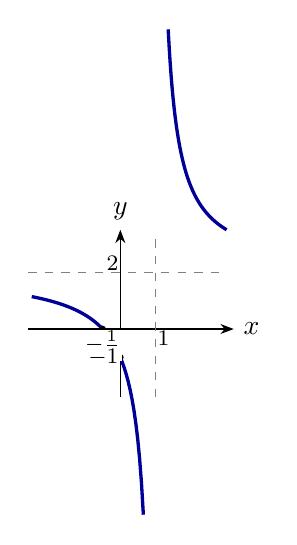
\begin{tikzpicture}[x=0.45cm,y=0.36cm,>=Stealth]
\draw[->] (-2.6,0)--(3.2,0) node[right] {$x$};
\draw[->] (0,-2.4)--(0,3.5) node[above] {$y$};
\draw[dashed,gray] (1,-2.4)--(1,3.3);
\draw[dashed,gray] (-2.6,2)--(3.0,2);
\draw[very thick,blue!60!black,domain=-2.5:0.65,samples=60] plot (\x,{(2*\x+1)/(\x-1)});
\draw[very thick,blue!60!black,domain=1.35:3.0,samples=60] plot (\x,{(2*\x+1)/(\x-1)});
\fill (0,-1) circle (1.2pt);\fill (-0.5,0) circle (1.2pt);
\node[below left,fill=white,inner sep=0.5pt] at (0,0) {\footnotesize $O$};
\node[below right,fill=white,inner sep=0.5pt] at (1,0) {\footnotesize $1$};
\node[above left,fill=white,inner sep=0.5pt] at (0,2) {\footnotesize $2$};
\node[below,fill=white,inner sep=0.5pt] at (-0.5,0) {\footnotesize $-\frac{1}{2}$};
\node[left,fill=white,inner sep=0.5pt] at (0,-1) {\footnotesize $-1$};
\end{tikzpicture}
\end{minipage}
\end{enumerate}

\newpage
\begin{enumerate}[start=7]
\item Một xưởng sản xuất thiết bị ước tính hàm chi phí trung bình (nghìn đồng) để sản xuất $x$ sản phẩm ($x>0$) là $\bar{C}(x)=\dfrac{1600}{x}+4x+50$. Xưởng cần sản xuất bao nhiêu sản phẩm để chi phí trung bình trên mỗi sản phẩm là thấp nhất?
\bonpa{$40$.}{$10$.}{$20$.}{$50$.}

\item Cho hình hộp chữ nhật $ABCD.A'B'C'D'$. Mệnh đề nào sau đây là đúng?
\bonpa{$\vec{BA}+\vec{BC}+\vec{BB'}=\vec{BD}$.}{$\vec{BA}+\vec{BC}+\vec{BB'}=\vec{AC'}$.}{$\vec{BA}+\vec{BC}+\vec{BB'}=\vec{B'D}$.}{$\vec{BA}+\vec{BC}+\vec{BB'}=\vec{BD'}$.}

\item Trong không gian $Oxyz$, cho hai điểm $A(1;-2;4)$ và $B(3;1;2)$. Tọa độ của vectơ $\vec{AB}$ là
\bonpa{$(2;3;-2)$.}{$(-2;-3;2)$.}{$(4;-1;6)$.}{$(2;-1;-2)$.}

\item Trong không gian $Oxyz$, cho tam giác $ABC$ có $A(2;1;-1)$, $B(1;0;3)$ và $C(3;2;4)$. Tọa độ trọng tâm $G$ của tam giác $ABC$ là
\bonpa{$(6;3;6)$.}{$(2;1;2)$.}{$(3;1;2)$.}{$(2;2;1)$.}

\item Trong không gian $Oxyz$, cho hai vectơ $\vec{u}=(1;0;-1)$ và $\vec{v}=(0;1;1)$. Số đo góc giữa hai vectơ $\vec{u}$ và $\vec{v}$ bằng
\bonpa{$60^\circ$.}{$45^\circ$.}{$120^\circ$.}{$135^\circ$.}

\item Trong không gian $Oxyz$, cho hai điểm $A(2;-1;3)$ và $B(4;1;2)$. Độ dài đoạn thẳng $AB$ bằng
\bonpa{$9$.}{$\sqrt{5}$.}{$\sqrt{13}$.}{$3$.}
\end{enumerate}

\vspace{3pt}
\section*{\large PHẦN II. Câu trắc nghiệm đúng hoặc sai}
\textit{Thí sinh trả lời từ câu 1 đến câu 4. Trong mỗi ý a), b), c), d) ở mỗi câu, thí sinh chọn đúng hoặc sai.}
\begin{enumerate}
\item Cho hàm số $y=f(x)=\dfrac{x^2+2x-2}{x-1}$.
\begin{enumerate}
\item Tập xác định của hàm số là $D=\mathbb{R}\setminus\{1\}$.
\item Đạo hàm của hàm số là $f'(x)=\dfrac{x^2-2x}{(x-1)^2}$ với mọi $x\ne 1$.
\item Đồ thị hàm số có đường tiệm cận xiên là đường thẳng $y=x-3$.
\item Khoảng cách giữa hai điểm cực trị của đồ thị hàm số bằng $2\sqrt{5}$.
\end{enumerate}
\end{enumerate}

\newpage
\begin{enumerate}[start=2]
\item Một cơ sở sản xuất thủ công mỗi ngày sản xuất $x$ mét vải lụa tơ tằm ($1\le x\le 18$). Tổng chi phí sản xuất $x$ mét vải lụa (tính bằng nghìn đồng) cho bởi hàm số $C(x)=x^3-3x^2-20x+500$. Mỗi ngày cơ sở bán hết sản phẩm với giá $220$ nghìn đồng/mét vải. Gọi $R(x)$ là doanh thu và $P(x)=R(x)-C(x)$ là lợi nhuận thu được khi bán $x$ mét vải lụa.
\begin{enumerate}
\item Chi phí cố định ban đầu của cơ sở (khi chưa sản xuất mét vải nào) là $500$ nghìn đồng.
\item Doanh thu của cơ sở khi bán $10$ mét vải lụa là $2200$ nghìn đồng.
\item Hàm lợi nhuận của cơ sở được biểu diễn bởi công thức $P(x)=-x^3+3x^2+240x-500$ (nghìn đồng).
\item Lợi nhuận lớn nhất mà cơ sở có thể đạt được trong một ngày là $1500$ nghìn đồng.
\end{enumerate}

\item Trong không gian $Oxyz$, cho ba điểm $A(2;1;0)$, $B(0;2;1)$ và $C(1;3;3)$.
\begin{enumerate}
\item Tọa độ của vectơ $\vec{AB}$ là $\vec{AB}=(-2;1;1)$.
\item Trọng tâm $G$ của tam giác $ABC$ có tọa độ là $G(1;2;1)$.
\item Độ dài hai đoạn thẳng $AB$ và $BC$ bằng nhau và bằng $\sqrt{6}$.
\item Tọa độ điểm $D$ để tứ giác $ABCD$ là hình bình hành là $D(3;2;2)$.
\end{enumerate}

\item Một chiếc đèn chùm trang trí có trọng lượng $P=60\text{ N}$ được treo vào trần nhà bằng ba sợi dây cáp không dãn có độ dài bằng nhau, nối từ trần nhà tại ba điểm $A, B, C$ tới móc treo đèn $O$. Ba điểm gắn dây trên trần nhà tạo thành tam giác đều và đối xứng nhau qua trục thẳng đứng đi qua $O$. Chọn hệ trục tọa độ $Oxyz$ có gốc tại $O$, tia $Oz$ hướng thẳng đứng lên trên. Khi đó trọng lực tác dụng lên đèn là $\vec{P}=(0;0;-60)$ (đơn vị: N). Các lực căng của ba sợi dây tác dụng lên móc treo $O$ lần lượt là $\vec{F}_1, \vec{F}_2, \vec{F}_3$ có cùng độ lớn $|\vec{F}_1|=|\vec{F}_2|=|\vec{F}_3|=F$.
\begin{enumerate}
\item Khi đèn ở trạng thái cân bằng thì $\vec{F}_1+\vec{F}_2+\vec{F}_3+\vec{P}=\vec{0}$.
\item Độ lớn hợp lực của ba lực căng dây bằng $60\text{ N}$.
\item Biết góc $\alpha$ giữa mỗi sợi dây cáp và phương thẳng đứng bằng $60^\circ$. Khi đó độ lớn của mỗi lực căng dây là $F=40\text{ N}$.
\item Khi kéo dài các sợi dây sao cho góc $\alpha$ giữa các sợi dây và phương thẳng đứng giảm đi thì độ lớn lực căng trên mỗi sợi dây sẽ tăng lên.
\end{enumerate}
\end{enumerate}

\vspace{3pt}
\section*{\large PHẦN III. Câu trắc nghiệm trả lời ngắn}
\textit{Thí sinh trả lời từ câu 1 đến câu 6. Mỗi câu trả lời đúng thí sinh được 0,5 điểm.}
\begin{enumerate}
\item Có bao nhiêu giá trị nguyên của tham số $m\in[-10;10]$ để hàm số $y=\dfrac{x+m}{x+4}$ đồng biến trên từng khoảng xác định?
\otraloi

\item Trong không gian $Oxyz$, cho hình hộp chữ nhật $ABCD.A'B'C'D'$ có đỉnh $A$ trùng với gốc tọa độ $O(0;0;0)$, đỉnh $B(4;0;0)$, đỉnh $D(0;6;0)$ và đỉnh $A'(0;0;3)$. Gọi $M$ là trung điểm của đoạn thẳng $B'C'$. Tìm tọa độ của điểm $M(x;y;z)$, sau đó tính giá trị của biểu thức $T=x+y+z$.
\otraloi
\end{enumerate}

\newpage
\begin{enumerate}[start=3]
\item Cho hàm số $y=\dfrac{x^2-4x+m}{x-1}$. Tìm số giá trị nguyên của tham số $m\in[-5;10]$ để đồ thị hàm số có hai điểm cực trị.
\otraloi

\item Trong không gian $Oxyz$ (với đơn vị đo trên các trục là mét), có hai thiết bị bay không người lái (drone) $A$ và $B$ đang bay thử nghiệm. Tại thời điểm $t$ giây ($t\ge 0$), vị trí của drone $A$ là $A(t;1;2t)$ và vị trí của drone $B$ là $B(5-t;-1;t)$. Khoảng cách ngắn nhất giữa hai drone trong quá trình bay bằng bao nhiêu mét?
\otraloi

\item Một chủ trang trại dự định làm một khu chuồng trại hình chữ nhật tiếp giáp với bờ một con sông thẳng để chăn nuôi gia cầm (bờ sông không cần rào). Trang trại còn muốn chia khu đất thành ba ô nhỏ hình chữ nhật bằng nhau bằng cách dựng thêm hai hàng rào ngăn phụ vuông góc với bờ sông (hình vẽ minh họa). Tổng chiều dài lưới rào thép hiện có là $120\text{ m}$. Diện tích lớn nhất của toàn bộ khu chuồng trại đó bằng bao nhiêu mét vuông?
\begin{center}
\begin{tikzpicture}[x=0.80cm,y=0.65cm,>=Stealth]
\fill[cyan!12] (-0.8,0) rectangle (9.8,-1.5);
\draw[thick,blue!60!black] (-0.8,0)--(9.8,0) node[right,black] {\footnotesize Bờ sông};
\node[blue!70!black] at (4.5,-0.75) {\textit{\footnotesize Dòng sông}};
\draw[line width=1.4pt,brown!60!black] (0,0)--(0,3.2)--(9.0,3.2)--(9.0,0);
\draw[line width=1.1pt,dashed,brown!60!black] (3.0,0)--(3.0,3.2);
\draw[line width=1.1pt,dashed,brown!60!black] (6.0,0)--(6.0,3.2);
\node at (1.5,1.6) {\footnotesize Ô 1};
\node at (4.5,1.6) {\footnotesize Ô 2};
\node at (7.5,1.6) {\footnotesize Ô 3};
\draw[<->] (-0.35,0)--(-0.35,3.2) node[midway,left] {\footnotesize $x$};
\draw[<->] (0,3.55)--(9.0,3.55) node[midway,above] {\footnotesize $y = 120 - 4x$};
\end{tikzpicture}
\par\smallskip{\footnotesize\textit{Hình minh họa sơ đồ khu chuồng trại ven bờ sông.}}
\end{center}
\otraloi

\item Một giàn khoan dầu $S$ ngoài khơi cách bờ biển thẳng một khoảng $SH=4\text{ km}$ ($H$ là hình chiếu vuông góc của $S$ lên bờ biển). Một nhà máy lọc dầu $A$ nằm trên bờ biển cách $H$ một khoảng $HA=9\text{ km}$. Người ta dự định lắp đặt đường ống dẫn dầu gồm hai đoạn: đoạn ống ngầm dưới đáy biển $SC$ đi từ giàn khoan $S$ đến một điểm $C$ trên bờ biển (nằm giữa $H$ và $A$), và đoạn ống $CA$ chạy dọc theo bờ biển từ $C$ đến nhà máy lọc dầu $A$ (hình vẽ minh họa). Biết chi phí lắp đặt mỗi kilômét đường ống ngầm dưới đáy biển là $50$ tỷ đồng, chi phí lắp đặt mỗi kilômét đường ống trên bờ biển là $30$ tỷ đồng. Tổng chi phí lắp đặt nhỏ nhất của đường ống dẫn dầu bằng bao nhiêu tỷ đồng?
\begin{center}
\begin{tikzpicture}[x=0.72cm,y=0.68cm,>=Stealth]
\fill[cyan!12] (-0.5,0) rectangle (9.8,2.6);
\draw[thick,blue!60!black] (-0.5,0)--(9.8,0) node[right,black] {\footnotesize Bờ biển};
\node[blue!70!black] at (5.0,2.0) {\textit{\footnotesize Biển khơi}};
\coordinate (S) at (1.2,2.3);
\coordinate (H) at (1.2,0);
\coordinate (C) at (4.2,0);
\coordinate (A) at (9.0,0);
\fill (S) circle (2pt) node[above] {$S$ (Giàn khoan)};
\fill (H) circle (2pt) node[below] {$H$};
\fill (C) circle (2pt) node[below] {$C$};
\fill (A) circle (2pt) node[below] {$A$ (Nhà máy)};
\draw[dashed] (S)--(H);
\draw (1.2,0.25)--(1.45,0.25)--(1.45,0);
\draw[line width=1.4pt,red!80!black] (S)--(C) node[midway,above,sloped] {\footnotesize ống dưới biển};
\draw[line width=1.6pt,orange!90!black] (C)--(A) node[midway,above] {\footnotesize ống trên bờ};
\draw[<->] (0.6,0)--(0.6,2.3) node[midway,left] {\footnotesize $4\text{ km}$};
\draw[<->] (1.2,-0.65)--(9.0,-0.65) node[midway,below] {\footnotesize $9\text{ km}$};
\end{tikzpicture}
\par\smallskip{\footnotesize\textit{Hình minh họa sơ đồ lắp đặt đường ống dẫn dầu.}}
\end{center}
\otraloi
\end{enumerate}
\begin{center}\textbf{---------------- HẾT ----------------}\end{center}

\newpage\pagestyle{answers}
\begin{center}\Large\textbf{BẢNG ĐÁP ÁN TỔNG HỢP}\end{center}
\textbf{Phần I. Trắc nghiệm nhiều phương án lựa chọn}
\begin{center}
\renewcommand{\arraystretch}{1.5}
\begin{tabular}{|c|*{12}{c|}}\hline
Câu & 1&2&3&4&5&6&7&8&9&10&11&12\\\hline
Đáp án & A & B & C & D & A & B & C & D & A & B & C & D \\\hline
\end{tabular}
\end{center}

\textbf{Phần II. Đúng hoặc sai}
\begin{center}
\renewcommand{\arraystretch}{1.4}
\begin{tabular}{|c|c|c|c|c|}\hline
Câu & a) & b) & c) & d)\\\hline
1 & Đ & Đ & S & Đ\\\hline
2 & Đ & Đ & Đ & S\\\hline
3 & Đ & S & Đ & Đ\\\hline
4 & Đ & Đ & Đ & S\\\hline
\end{tabular}
\end{center}

\textbf{Phần III. Trả lời ngắn}
\begin{center}
\renewcommand{\arraystretch}{1.5}
\begin{tabular}{|c|c|c|c|c|c|c|}\hline
Câu & 1 & 2 & 3 & 4 & 5 & 6\\\hline
Đáp án & 14 & 10 & 7 & 3 & 900 & 430 \\\hline
\end{tabular}
\end{center}

\textbf{Thang điểm dùng cho đề ôn tập:}
\begin{itemize}[leftmargin=*,itemsep=3pt]
\item Phần I: mỗi câu đúng $0{,}25$ điểm; tối đa $3$ điểm.
\item Phần II: mỗi câu có 4 ý. Đúng 1, 2, 3, 4 ý lần lượt được $0{,}1$; $0{,}25$; $0{,}5$; $1$ điểm. Tối đa $4$ điểm.
\item Phần III: mỗi câu đúng $0{,}5$ điểm; tối đa $3$ điểm.
\end{itemize}
\textbf{Phạm vi:} Bài 1–5 (ứng dụng đạo hàm và khảo sát hàm số), Bài 6–8 (vectơ và tọa độ trong không gian).
Tổng điểm $10$; thời gian $90$ phút.

\newpage
\begin{center}\Large\textbf{HƯỚNG DẪN GIẢI CHI TIẾT}\end{center}
\section*{\large Phần I}
\loigiai{Câu 1. Chọn A.}
Ta có $y'=3x^2-6x=3x(x-2)$.
Xét $y'<0\Leftrightarrow 3x(x-2)<0\Leftrightarrow 0<x<2$.
Vậy hàm số đã cho nghịch biến trên khoảng $(0;2)$.

\loigiai{Câu 2. Chọn B.}
Ta có $y'=x^2-4x+3=(x-1)(x-3)$.
Phương trình $y'=0\Leftrightarrow x=1$ hoặc $x=3$.
Đạo hàm cấp hai: $y''=2x-4$.
Tại $x=1$, ta có $y''(1)=-2<0$, suy ra $x=1$ là điểm cực đại của hàm số.
Tại $x=3$, ta có $y''(3)=2>0$, suy ra $x=3$ là điểm cực tiểu của hàm số.

\loigiai{Câu 3. Chọn C.}
Hàm số liên tục trên đoạn $[0;2]$. Đạo hàm: $f'(x)=3x^2-3=3(x-1)(x+1)$.
Trên đoạn $[0;2]$, ta có $f'(x)=0\Leftrightarrow x=1$.
Tính các giá trị:
$f(0)=5$; $f(1)=1^3-3\cdot 1+5=3$; $f(2)=2^3-3\cdot 2+5=7$.
Vậy giá trị nhỏ nhất của hàm số trên đoạn $[0;2]$ là $\min_{[0;2]}f(x)=3$ (đạt tại $x=1$).

\loigiai{Câu 4. Chọn D.}
Ta có $\lim_{x\to (-3)^+}\dfrac{2x-1}{x+3}=-\infty$ và $\lim_{x\to (-3)^-}\dfrac{2x-1}{x+3}=+\infty$ nên đường thẳng $x=-3$ là tiệm cận đứng.
Lại có $\lim_{x\to\pm\infty}\dfrac{2x-1}{x+3}=2$ nên đường thẳng $y=2$ là tiệm cận ngang.
Giao điểm của hai đường tiệm cận có tọa độ là $(-3;2)$.

\loigiai{Câu 5. Chọn A.}
Thực hiện phép chia đa thức: $\dfrac{x^2+2x-1}{x-1}=x+3+\dfrac{2}{x-1}$.
Vì $\lim_{x\to\pm\infty}\left[\dfrac{x^2+2x-1}{x-1}-(x+3)\right]=\lim_{x\to\pm\infty}\dfrac{2}{x-1}=0$ nên đường tiệm cận xiên của đồ thị hàm số là đường thẳng $y=x+3$.

\loigiai{Câu 6. Chọn B.}
Dựa vào hình vẽ, đồ thị có đường tiệm cận đứng $x=1$ và đường tiệm cận ngang $y=2$.
Đồ thị đi qua điểm cắt trục tung $(0;-1)$ và cắt trục hoành tại $\left(-\dfrac{1}{2};0\right)$.
Trong các phương án đã cho:
Chỉ có hàm số $y=\dfrac{2x+1}{x-1}$ thỏa mãn tiệm cận ngang $y=2$, đi qua $(0;-1)$ và nghịch biến trên từng khoảng xác định.

\loigiai{Câu 7. Chọn C.}
Xét hàm chi phí trung bình $\bar{C}(x)=\dfrac{1600}{x}+4x+50$ với $x>0$.
Đạo hàm: $\bar{C}'(x)=-\dfrac{1600}{x^2}+4$.
Cho $\bar{C}'(x)=0\Leftrightarrow \dfrac{1600}{x^2}=4\Leftrightarrow x^2=400\Rightarrow x=20$ (do $x>0$).
Lập bảng biến thiên thấy hàm số $\bar{C}(x)$ đạt giá trị nhỏ nhất tại $x=20$.
Vậy xưởng cần sản xuất $20$ sản phẩm.

\loigiai{Câu 8. Chọn D.}
Theo quy tắc hình hộp, ba vectơ cạnh xuất phát từ cùng một đỉnh $B$ của hình hộp chữ nhật $ABCD.A'B'C'D'$ có tổng bằng vectơ đường chéo xuất phát từ đỉnh đó: $\vec{BA}+\vec{BC}+\vec{BB'}=\vec{BD'}$.

\loigiai{Câu 9. Chọn A.}
Tọa độ của vectơ $\vec{AB}$ là:
$\vec{AB}=(x_B-x_A;y_B-y_A;z_B-z_A)=(3-1;1-(-2);2-4)=(2;3;-2)$.

\loigiai{Câu 10. Chọn B.}
Tọa độ trọng tâm $G$ của tam giác $ABC$ là:
$x_G=\dfrac{2+1+3}{3}=2$, $y_G=\dfrac{1+0+2}{3}=1$, $z_G=\dfrac{-1+3+4}{3}=2$.
Vậy $G(2;1;2)$.

\loigiai{Câu 11. Chọn C.}
Tích vô hướng của hai vectơ:
$\vec{u}\cdot\vec{v}=1\cdot 0+0\cdot 1+(-1)\cdot 1=-1$.
Độ dài của hai vectơ:
$|\vec{u}|=\sqrt{1^2+0^2+(-1)^2}=\sqrt{2}$, $|\vec{v}|=\sqrt{0^2+1^2+1^2}=\sqrt{2}$.
Cosin góc giữa hai vectơ:
$\cos(\vec{u},\vec{v})=\dfrac{\vec{u}\cdot\vec{v}}{|\vec{u}|\cdot|\vec{v}|}=\dfrac{-1}{\sqrt{2}\cdot\sqrt{2}}=-\dfrac{1}{2}$.
Suy ra góc giữa hai vectơ bằng $120^\circ$.

\loigiai{Câu 12. Chọn D.}
Độ dài đoạn thẳng $AB$ là:
$AB=\sqrt{(4-2)^2+(1-(-1))^2+(2-3)^2}=\sqrt{4+4+1}=3$.

\newpage
\section*{\large Phần II}
\loigiai{Câu 1.}
a) Hàm số xác định khi mẫu số $x-1\ne 0\Leftrightarrow x\ne 1$. Do đó tập xác định $D=\mathbb{R}\setminus\{1\}$. Mệnh đề đúng.\\
b) Đạo hàm:
$f'(x)=\dfrac{(2x+2)(x-1)-(x^2+2x-2)}{(x-1)^2}=\dfrac{2x^2-2-x^2-2x+2}{(x-1)^2}=\dfrac{x^2-2x}{(x-1)^2}$. Mệnh đề đúng.\\
c) Phân tích: $\dfrac{x^2+2x-2}{x-1}=x+3+\dfrac{1}{x-1}$.
Vì $\lim_{x\to\pm\infty}[f(x)-(x+3)]=0$ nên đường tiệm cận xiên là $y=x+3$, chứ không phải $y=x-3$. Mệnh đề sai.\\
d) Cho $f'(x)=0\Leftrightarrow x(x-2)=0\Leftrightarrow x_1=0$ hoặc $x_2=2$.
Với $x=0\Rightarrow y=2$, điểm cực trị thứ nhất là $A(0;2)$.
Với $x=2\Rightarrow y=6$, điểm cực trị thứ hai là $B(2;6)$.
Khoảng cách giữa hai điểm cực trị:
$AB=\sqrt{(2-0)^2+(6-2)^2}=\sqrt{4+16}=\sqrt{20}=2\sqrt{5}$. Mệnh đề đúng.

\loigiai{Câu 2.}
a) Chi phí cố định là chi phí khi $x=0$: $C(0)=500$ (nghìn đồng). Mệnh đề đúng.\\
b) Doanh thu khi bán $10$ mét vải lụa là: $R(10)=220\cdot 10=2200$ (nghìn đồng). Mệnh đề đúng.\\
c) Hàm lợi nhuận thu được khi bán $x$ mét vải:
$P(x)=R(x)-C(x)=220x-(x^3-3x^2-20x+500)=-x^3+3x^2+240x-500$ (nghìn đồng). Mệnh đề đúng.\\
d) Đạo hàm của hàm lợi nhuận:
$P'(x)=-3x^2+6x+240=-3(x^2-2x-80)=-3(x-10)(x+8)$.
Trên đoạn $[1;18]$, phương trình $P'(x)=0\Leftrightarrow x=10$.
Ta thấy $P'(x)>0$ với $x\in[1;10)$ và $P'(x)<0$ với $x\in(10;18]$, do đó hàm lợi nhuận đạt giá trị lớn nhất tại $x=10$.
Lợi nhuận lớn nhất là:
$P(10)=-10^3+3\cdot 10^2+240\cdot 10-500=-1000+300+2400-500=1200$ (nghìn đồng).
Mệnh đề nói lợi nhuận lớn nhất là $1500$ nghìn đồng là sai. Mệnh đề sai.

\loigiai{Câu 3.}
a) Ta có $\vec{AB}=(0-2;2-1;1-0)=(-2;1;1)$. Mệnh đề đúng.\\
b) Tọa độ trọng tâm $G$ của tam giác $ABC$ là:
$x_G=\dfrac{2+0+1}{3}=1$, $y_G=\dfrac{1+2+3}{3}=2$, $z_G=\dfrac{0+1+3}{3}=\dfrac{4}{3}$.
Tọa độ đúng là $G\left(1;2;\dfrac{4}{3}\right)$, do đó mệnh đề sai.\\
c) Ta có $\vec{AB}=(-2;1;1)\Rightarrow AB=\sqrt{(-2)^2+1^2+1^2}=\sqrt{6}$.
Lại có $\vec{BC}=(1-0;3-2;3-1)=(1;1;2)\Rightarrow BC=\sqrt{1^2+1^2+2^2}=\sqrt{6}$.
Vậy $AB=BC=\sqrt{6}$. Mệnh đề đúng.\\
d) Tứ giác $ABCD$ là hình bình hành khi và chỉ khi $\vec{AD}=\vec{BC}$.
Gọi $D(x;y;z)$, ta có $\vec{AD}=(x-2;y-1;z-0)$.
Mà $\vec{BC}=(1;1;2)$ nên $\begin{cases}x-2=1\\y-1=1\\z=2\end{cases}\Leftrightarrow\begin{cases}x=3\\y=2\\z=2\end{cases}\Rightarrow D(3;2;2)$. Mệnh đề đúng.

\loigiai{Câu 4.}
a) Khi chiếc đèn trang trí ở trạng thái cân bằng thì hợp lực của ba lực căng cáp tác dụng lên móc treo phải triệt tiêu trọng lực của đèn, tức là $\vec{F}_1+\vec{F}_2+\vec{F}_3+\vec{P}=\vec{0}$. Mệnh đề đúng.\\
b) Từ hệ thức cân bằng suy ra $\vec{F}_1+\vec{F}_2+\vec{F}_3=-\vec{P}$.
Do đó độ lớn hợp lực của ba lực căng là $|\vec{F}_1+\vec{F}_2+\vec{F}_3|=|-\vec{P}|=60\text{ N}$. Mệnh đề đúng.\\
c) Do ba điểm treo đối xứng nhau qua trục thẳng đứng $Oz$, hình chiếu của ba lực căng lên trục $Oz$ đều bằng $F\cos\alpha$.
Hợp lực theo phương thẳng đứng cân bằng với trọng lực nên:
$3F\cos\alpha=60\Rightarrow F=\dfrac{20}{\cos\alpha}$.
Với $\alpha=60^\circ$, ta có $\cos 60^\circ=\dfrac{1}{2}$, do đó $F=\dfrac{20}{1/2}=40\text{ N}$. Mệnh đề đúng.\\
d) Từ công thức $F=\dfrac{20}{\cos\alpha}$, khi góc $\alpha$ giảm đi (với $0<\alpha<90^\circ$) thì $\cos\alpha$ tăng lên, dẫn đến độ lớn lực căng $F$ giảm đi. Do đó mệnh đề nói lực căng tăng lên là sai. Mệnh đề sai.

\newpage
\section*{\large Phần III}
\loigiai{Câu 1.}
Tập xác định $D=\mathbb{R}\setminus\{-4\}$.
Đạo hàm: $y'=\dfrac{1\cdot 4-1\cdot m}{(x+4)^2}=\dfrac{4-m}{(x+4)^2}$.
Hàm số đồng biến trên từng khoảng xác định khi và chỉ khi $y'>0,\ \forall x\ne -4\Leftrightarrow 4-m>0\Leftrightarrow m<4$.
Vì $m\in[-10;10]$ và $m\in\mathbb{Z}$ nên $m\in\{-10;-9;-8;\dots;2;3\}$.
Số giá trị nguyên của tham số $m$ thỏa mãn là:
$3-(-10)+1=14$.

\loigiai{Câu 2.}
Vì hình hộp chữ nhật có ba cạnh xuất phát từ đỉnh $A(0;0;0)$ nằm trên ba trục tọa độ:
$\vec{AB}=(4;0;0)$, $\vec{AD}=(0;6;0)$, $\vec{AA'}=(0;0;3)$.
Suy ra tọa độ các đỉnh:
$B(4;0;0)$, $D(0;6;0)$, $A'(0;0;3)$.
Đỉnh $C$ thuộc mặt phẳng đáy $(Oxy)$ có $\vec{AC}=\vec{AB}+\vec{AD}=(4;6;0)\Rightarrow C(4;6;0)$.
Đỉnh $B'$ có tọa độ $\vec{OB'}=\vec{OB}+\vec{AA'}=(4;0;3)\Rightarrow B'(4;0;3)$.
Đỉnh $C'$ có tọa độ $\vec{OC'}=\vec{OC}+\vec{AA'}=(4;6;3)\Rightarrow C'(4;6;3)$.
Điểm $M$ là trung điểm của đoạn thẳng $B'C'$ nên tọa độ của $M$ là:
$x_M=\dfrac{4+4}{2}=4$, $y_M=\dfrac{0+6}{2}=3$, $z_M=\dfrac{3+3}{2}=3$.
Vậy $M(4;3;3)$, suy ra $T=x+y+z=4+3+3=10$.

\loigiai{Câu 3.}
Tập xác định $D=\mathbb{R}\setminus\{1\}$.
Đạo hàm:
$y'=\dfrac{(2x-4)(x-1)-(x^2-4x+m)}{(x-1)^2}=\dfrac{x^2-2x+4-m}{(x-1)^2}$.
Đồ thị hàm số có hai điểm cực trị khi và chỉ khi tam thức bậc hai $g(x)=x^2-2x+4-m=0$ có hai nghiệm phân biệt khác $1$:
$\begin{cases}\Delta'=(-1)^2-(4-m)=m-3>0\\ g(1)=1^2-2\cdot 1+4-m=3-m\ne 0\end{cases}\Leftrightarrow m>3$.
Kết hợp với $m\in[-5;10]$ và $m\in\mathbb{Z}$, ta nhận các giá trị $m\in\{4;5;6;7;8;9;10\}$.
Vậy có tất cả $7$ giá trị nguyên của tham số $m$ thỏa mãn yêu cầu bài toán.

\loigiai{Câu 4.}
Tại thời điểm $t\ge 0$, vị trí của hai drone lần lượt là $A(t;1;2t)$ và $B(5-t;-1;t)$.
Vectơ nối vị trí hai drone là:
$\vec{AB}=(5-t-t;-1-1;t-2t)=(5-2t;-2;-t)$.
Bình phương khoảng cách giữa hai drone tại thời điểm $t$ là:
$d^2(t)=(5-2t)^2+(-2)^2+(-t)^2=(25-20t+4t^2)+4+t^2=5t^2-20t+29$.
Biến đổi tam thức bậc hai:
$d^2(t)=5(t^2-4t+4)+9=5(t-2)^2+9\ge 9,\ \forall t\ge 0$.
Dấu đẳng thức xảy ra khi $t=2$ (thỏa mãn $t\ge 0$).
Vậy khoảng cách ngắn nhất giữa hai drone trong quá trình bay là $d_{\min}=\sqrt{9}=3\text{ mét}$.

\loigiai{Câu 5.}
Gọi chiều rộng của khu đất (độ dài của mỗi đoạn rào vuông góc với bờ sông) là $x\text{ (m)}$ với điều kiện $x>0$.
Vì có hai hàng rào ngăn phụ và hai hàng rào biên nên có tất cả $4$ đoạn rào vuông góc với bờ sông, tổng độ dài là $4x\text{ (m)}$.
Độ dài hàng rào chạy dọc theo bờ đối diện bờ sông là:
$y=120-4x\text{ (m)}$.
Điều kiện: $120-4x>0\Leftrightarrow 0<x<30$.
Diện tích của toàn bộ khu chuồng trại là:
$S(x)=x\cdot y=x(120-4x)=120x-4x^2\text{ (m}^2\text{)}$.
Đạo hàm: $S'(x)=120-8x$.
Cho $S'(x)=0\Leftrightarrow 8x=120\Leftrightarrow x=15\text{ m}$.
Vì $S''(x)=-8<0$ nên hàm số $S(x)$ đạt cực đại và là giá trị lớn nhất tại $x=15\in(0;30)$.
Khi đó chiều dài của khu chuồng trại là $y=120-4\cdot 15=60\text{ m}$.
Diện tích lớn nhất của khu chuồng trại là:
$S_{\max}=S(15)=15\cdot 60=900\text{ m}^2$.

\loigiai{Câu 6.}
Đặt khoảng cách từ hình chiếu $H$ đến điểm cập bờ $C$ là $HC=x\text{ (km)}$ với $0\le x\le 9$.
Vì tam giác $SHC$ vuông tại $H$ nên độ dài đoạn ống ngầm dưới đáy biển là:
$SC=\sqrt{SH^2+HC^2}=\sqrt{4^2+x^2}=\sqrt{x^2+16}\text{ (km)}$.
Độ dài đoạn ống dẫn chạy trên bờ biển từ $C$ đến nhà máy lọc dầu $A$ là:
$CA=HA-HC=9-x\text{ (km)}$.
Tổng chi phí lắp đặt toàn bộ đường ống dẫn dầu là hàm số theo $x$:
$f(x)=50\sqrt{x^2+16}+30(9-x)\quad (\text{tỷ đồng})$.
Xét hàm số $f(x)$ trên đoạn $[0;9]$. Đạo hàm:
$f'(x)=\dfrac{50x}{\sqrt{x^2+16}}-30$.
Cho $f'(x)=0\Leftrightarrow \dfrac{50x}{\sqrt{x^2+16}}=30\Leftrightarrow \dfrac{5x}{\sqrt{x^2+16}}=3$
$\Leftrightarrow 25x^2=9(x^2+16)\Leftrightarrow 16x^2=144\Leftrightarrow x^2=9\Rightarrow x=3\text{ (do } x\ge 0\text{)}$.
Giá trị $x=3\in[0;9]$.
Ta tính giá trị của hàm chi phí tại các điểm biên và điểm dừng:
$f(0)=50\sqrt{16}+30\cdot 9=200+270=470\text{ tỷ đồng}$;
$f(9)=50\sqrt{9^2+16}+30\cdot 0=50\sqrt{97}\approx 492{,}44\text{ tỷ đồng}$;
$f(3)=50\sqrt{3^2+16}+30(9-3)=50\cdot 5+30\cdot 6=250+180=430\text{ tỷ đồng}$.
So sánh ba giá trị trên, ta thấy chi phí lắp đặt nhỏ nhất là $430$ tỷ đồng (đạt được khi đặt trạm cập bờ $C$ cách $H$ một khoảng $3\text{ km}$).

\end{document}
